\documentclass[runningheads]{llncs}
%
\usepackage{graphicx}
\usepackage{amsmath}
\usepackage{amssymb}
\usepackage{booktabs}
\usepackage{tikz}
\usetikzlibrary{arrows.meta,positioning,fit,backgrounds}
\usepackage{microtype}
\usepackage[colorlinks=true,linkcolor=black,citecolor=black,urlcolor=blue,breaklinks=true]{hyperref}
\renewcommand\UrlFont{\color{blue}\rmfamily}
%
\begin{document}
%
% Prioritize never overflowing the margin over perfectly even interword
% spacing -- several dense \texttt clusters (parameter names, model IDs)
% were causing slight overfull-hbox bleeds that targeted \allowbreak
% fixes weren't reliably catching.
\sloppy
%
\title{GAVE2 Challenge Technical Report: aaronteam}
%
\titlerunning{GAVE2 Technical Report: aaronteam}
%
\author{Aaron Ajit}
%
\authorrunning{A. Ajit}
%
\institute{Independent participant, GAVE2 Challenge (MICCAI 2026 OMIA Workshop)\\
\email{aaronajit@gmail.com}}
%
\maketitle
%
\begin{abstract}
This report describes team aaronteam's submission to the GAVE2 (Generalized
Analysis of Vessels in Eye, Edition 2) challenge preliminary round. Our
pipeline builds on the official CMRRWNet baseline and its RRWNet backbone
\cite{morano2024rrwnet}, adding a topology-aware soft-clDice loss
\cite{shit2021cldice}, an asymmetric artery/vein loss weighting scheme, a
multi-seed cross-validation ensemble (11--12 members across three
independent random partitions, one member down-weighted), horizontal-flip
test-time augmentation, and a
SegFormer-based optic disc detector \cite{xie2021segformer} for Task 3
biomarker extraction. We additionally found and corrected an unvalidated
assumption in the baseline pipeline (Task 3 should be sourced from Task 1's
segmentation, not Task 2's), and found empirically that Task 3's biomarker
accuracy benefits from a smaller, sharper segmentation ensemble than the one
used for Task 1/Task 2 scoring, since over-averaging blurs thin vessel
structure. Our final submission scored 7.06756 (round score), placing in the
top 30 of the preliminary leaderboard.

\medskip\noindent\textbf{Keywords:} Retinal vessel segmentation
$\cdot$ Artery/vein classification $\cdot$ Topology-preserving loss
$\cdot$ Ensemble learning $\cdot$ Vascular biomarkers.
\end{abstract}
%
%
%
\section{Proposed Method}

\subsection{Model Framework}

Figure~\ref{fig:pipeline} shows the overall pipeline. Task 1 (CFP-only
artery/vein segmentation) uses RRWNet \cite{morano2024rrwnet}, a single-branch
U-Net-style encoder-decoder followed by a recursive refinement module applied
iteratively. Task 2 (CFP+FFA artery/vein segmentation) uses CMRRWNet, the
official GAVE2 baseline architecture, which extends RRWNet with two
additional encoder branches for the early- and late-phase FFA images and an
SE-gated channel-attention fusion module that combines the three branches at
four encoder scales before a shared decoder and the same recursive refinement
module used in Task 1. Task 3 (vascular biomarker regression) is not a
learned model -- it computes five biomarkers (AVR, artery/vein density,
artery/vein fractal dimension) directly from a segmentation-model's
artery/vein masks plus an optic disc mask from a separate pretrained
detector.

\begin{figure}[t]
\centering
\resizebox{0.95\textwidth}{!}{%
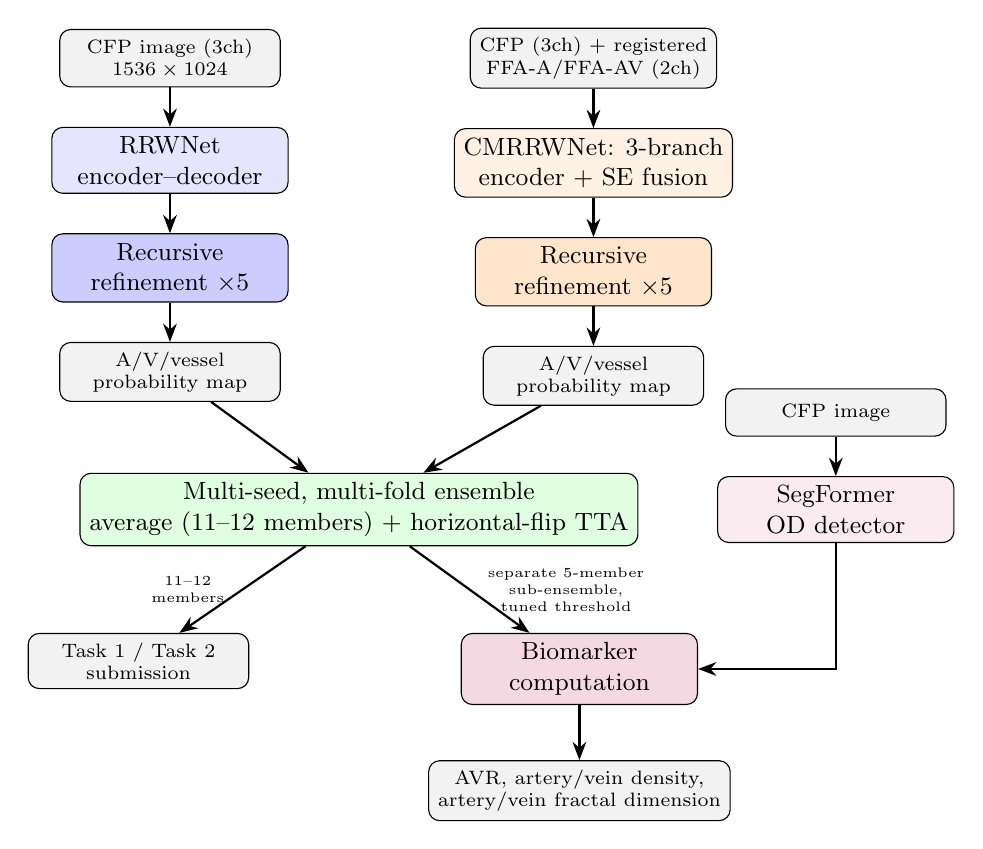
\begin{tikzpicture}[
  box/.style={draw, rounded corners, minimum height=0.8cm, minimum width=3.0cm, align=center, font=\small},
  io/.style={draw, rounded corners, minimum height=0.6cm, minimum width=2.8cm, align=center, font=\scriptsize, fill=gray!10},
  arr/.style={-Stealth, thick},
  lbl/.style={font=\tiny, align=center}
]
  % Task 1 column (left)
  \node[io] (cfp1) {CFP image (3ch)\\$1536\times1024$};
  \node[box, below=0.5cm of cfp1, fill=blue!10] (rrwnet) {RRWNet\\encoder--decoder};
  \node[box, below=0.5cm of rrwnet, fill=blue!20] (refine1) {Recursive\\refinement $\times5$};
  \node[io, below=0.5cm of refine1] (out1) {A/V/vessel\\probability map};

  \draw[arr] (cfp1) -- (rrwnet);
  \draw[arr] (rrwnet) -- (refine1);
  \draw[arr] (refine1) -- (out1);

  % Task 2 column (right)
  \node[io, right=2.4cm of cfp1] (cfp2) {CFP (3ch) + registered\\FFA-A/FFA-AV (2ch)};
  \node[box, below=0.5cm of cfp2, fill=orange!10] (cmrrwnet) {CMRRWNet: 3-branch\\encoder + SE fusion};
  \node[box, below=0.5cm of cmrrwnet, fill=orange!20] (refine2) {Recursive\\refinement $\times5$};
  \node[io, below=0.5cm of refine2] (out2) {A/V/vessel\\probability map};

  \draw[arr] (cfp2) -- (cmrrwnet);
  \draw[arr] (cmrrwnet) -- (refine2);
  \draw[arr] (refine2) -- (out2);

  % Ensemble, centered between the two output nodes
  \node[box, below=0.9cm of out1, xshift=2.4cm, fill=green!12, minimum width=5.6cm] (ens) {Multi-seed, multi-fold ensemble\\average (11--12 members) + horizontal-flip TTA};
  \draw[arr] (out1) -- (ens);
  \draw[arr] (out2) -- (ens);

  % Split: Task1/Task2 submission (left) vs. a separate, smaller Task3
  % sub-ensemble (right) -- offsets kept large/symmetric on purpose so the
  % two branches can't collide regardless of exact box widths.
  \node[io, below=1.1cm of ens, xshift=-2.8cm] (t1t2out) {Task 1 / Task 2\\submission};
  \node[box, below=1.1cm of ens, xshift=2.8cm, fill=purple!15] (biomarker) {Biomarker\\computation};
  \draw[arr] (ens) -- node[lbl, left, xshift=-0.1cm] {11--12\\members} (t1t2out);
  \draw[arr] (ens) -- node[lbl, right, xshift=0.1cm] {separate 5-member\\sub-ensemble,\\tuned threshold} (biomarker);

  % Optic disc branch: placed well clear of the split above (same row as
  % ens, off to the right) so it can't compete for space with t1t2out/biomarker.
  \node[box, right=1.0cm of ens, fill=purple!8] (segformer) {SegFormer\\OD detector};
  \node[io, above=0.5cm of segformer] (cfp3) {CFP image};
  \draw[arr] (cfp3) -- (segformer);
  \draw[arr] (segformer) |- (biomarker);

  \node[io, below=0.7cm of biomarker] (out3) {AVR, artery/vein density,\\artery/vein fractal dimension};
  \draw[arr] (biomarker) -- (out3);

\end{tikzpicture}%
}
\caption{Overview of the full pipeline. Task 1 (top) and Task 2 (middle) share
the RRWNet recursive-refinement backbone; Task 2 adds a 3-branch encoder with
SE-gated fusion for the extra FFA modality. Both feed a multi-seed,
multi-fold ensemble with horizontal-flip TTA. Task 3 (bottom) computes
biomarkers from a \emph{separate}, smaller ensemble of Task 1 predictions
(see Sect.~\ref{sec:postprocessing}) plus an independently-trained optic disc
detector.}
\label{fig:pipeline}
\end{figure}

\subsection{Structure Detail Description}

\textbf{Backbone.} Both tasks use the same recursive-refinement decoder
design from RRWNet: an initial U-Net-style prediction is iteratively refined
by a shared, weight-tied refinement block (\texttt{second\_u}) applied 5
times at both train and inference time. Later refinement iterations are
weighted more heavily in the loss (Eq.~\ref{eq:rrloss}), reflecting that
later iterations are strictly more refined. All layer weights for the shared
recursive-refinement module are identical across iterations (a single set of
weights applied repeatedly, not 5 independent decoder stages).

\textbf{Task 1 (RRWNet, 3-channel input).} A single encoder path
(\texttt{conv1--conv5}) at base channel width 64, U-Net decoder
(\texttt{upconv1--upconv4}, \texttt{conv6--conv9}), producing a 3-channel
logit map (artery, vessel-union, vein). Warm-started from HRF-pretrained
weights (\texttt{j-morano/rrwnet-hrf}, HuggingFace) before fine-tuning on
GAVE2 data.

\textbf{Task 2 (CMRRWNet, 5-channel input).} Three parallel encoders (RGB
CFP, early-phase FFA, late-phase FFA), fused at four encoder scales via an
SE-gated channel-attention additive fusion module (\texttt{Asy\_fusion1--4}
in the baseline code), feeding the same decoder/refinement structure as Task
1. We warm-start Task 2's RGB encoder, decoder, and recursive-refinement
weights directly from a trained Task 1 checkpoint (180/180 matching tensors
transferred by name, verified); the two FFA-branch encoders and their
attention layers have no Task 1 counterpart and start from random
initialization.

\textbf{Loss function.} Both tasks use the same composite loss:
\begin{equation}
\mathcal{L} = \mathcal{L}_{\text{RR}} + \lambda_{\text{cl}}\,\mathcal{L}_{\text{clDice}}
\label{eq:total_loss}
\end{equation}
where $\mathcal{L}_{\text{RR}}$ is a weighted sum of per-channel BCE losses
across the model's $M{+}2$ predictions: one initial (non-refined) prediction
from the base U-Net, plus $M{+}1$ recursive-refinement predictions ($M{=}5$
explicit refinement iterations, plus one further application of the same
refinement module prior to that loop). The initial prediction is weighted
separately, and the remaining $k{=}M{+}1$ refinement predictions are
weighted $1,2,\dots,k$ (later, more-refined predictions weighted more
heavily), normalized so the weights sum to 1:
\begin{equation}
\mathcal{L}_{\text{RR}} = \mathcal{L}_1 + \frac{1}{Z}\sum_{j=1}^{k} j \cdot \mathcal{L}_{j+1},
\qquad k = M{+}1, \quad Z = \tfrac{1}{2}k(k{+}1),
\label{eq:rrloss}
\end{equation}
$\mathcal{L}_i$ being the per-prediction BCE3 loss (independent weighted BCE
on artery, vessel-union, and vein channels, with the vein channel given its
own, higher positive-class weight than artery -- $\texttt{pos\_weight}=5.0$,
$\texttt{vein\_pos\_weight}=6.0$ -- since vessels are a small minority class
and empirically the vein channel needed extra weight to avoid
under-segmentation). $\mathcal{L}_{\text{clDice}}$ is soft-clDice
\cite{shit2021cldice}, a differentiable topology-preserving loss computed on
soft-skeletonized artery and vein predictions:
\begin{equation}
\mathcal{L}_{\text{clDice}} = 1 - \frac{2\,T_{\text{prec}}\,T_{\text{sens}}}{T_{\text{prec}} + T_{\text{sens}}},
\end{equation}
applied separately to the artery and vein channels of the final refinement
iteration only, and combined with an asymmetric weighting
($\texttt{vein\_topology\_ratio}=1.3$) since the vein channel showed
persistently worse topology (connectivity) metrics than artery in early
experiments. We use $\lambda_{\text{cl}} = 0.3$.

\textbf{Task 3 (vascular biomarkers).} Not a trained network. Given an
artery/vein segmentation mask and an optic disc mask, we compute: (i) CRAE
and CRVE (central retinal artery/vein equivalent) via the revised Knudtson
formula \cite{knudtson2003revised} on the six widest artery/vein segments
within the SIVA Zone-C annulus around the optic disc, (ii) AVR as their
ratio, (iii) artery/vein vessel density within Zone-C, and (iv) artery/vein
fractal dimension via box-counting on the whole-image vessel skeleton. The
optic disc mask comes from a SegFormer model \cite{xie2021segformer}
pretrained on REFUGE for disc/cup segmentation
(\texttt{pamixsun/\allowbreak segformer\_\allowbreak for\_\allowbreak optic\_\allowbreak disc\_\allowbreak cup\_\allowbreak segmentation}, used
frozen, no fine-tuning), replacing the challenge baseline's MNet\_DeepCDR
detector.

\subsection{Input/Output (Data Flow)}

CFP images are $1536\times1024$ RGB, normalized to $[0,1]$. FFA images
(early and late phase, grayscale) are not natively aligned to the CFP image
for a given case -- we verified this empirically (mean displacement
$\approx256$px under naive ORB matching, i.e.\ noise) -- so they are
registered to the CFP image with MINIMA \cite{ren2025minima}
(SuperPoint+LightGlue feature matching) before being stacked as two
additional input channels for Task 2 (5 channels total: 3 RGB + FFA-early +
FFA-late).

Training uses random square crops (see Sect.~\ref{sec:preprocessing}) rather
than the full image, since downscaling the whole image loses the thin-vessel
detail that the topology metrics are sensitive to. Inference uses
overlapping-tile sliding-window prediction at full native resolution, with
tile/stride chosen per task to fit the available GPU memory (Task 1:
$384\times384$/288; Task 2: $320\times320$/288). Output is always a
3-channel probability map in [artery, vessel-union, vein] channel order,
matching the label convention.

Task 3's input is an artery/vein mask (from a specific sub-ensemble of Task 1
models, see Sect.~\ref{sec:postprocessing}) plus the original CFP image (for
optic disc detection); its output is five scalar biomarker values per image.

%
\section{Experiment Configuration}

\subsection{Datasets}
GAVE2 preliminary dataset: 50 labeled training cases (color fundus
photograph, early- and late-phase FFA, pixel-level artery/vein segmentation
ground truth, a field-of-view ROI mask, and ground-truth biomarker values)
and 50 unlabeled cases used for leaderboard evaluation. Beyond the challenge
data, we use two sets of publicly available pretrained weights: HRF-pretrained
weights for RRWNet's initialization (Sect.~1.2) and REFUGE-pretrained
weights for the SegFormer optic disc detector (Sect.~1.2); no other
external training data was used.

\subsection{Datasets Split Method}
5-fold cross-validation, plain random splitting (no camera-vendor
stratification, since no vendor metadata ships with the dataset). To build a
larger, more diverse ensemble than a single 5-fold partition allows, we
generated three independent 5-fold partitions using different random seeds
(77, 101, 202) and trained a model on each fold of each partition, using
folds from partitions the model was never validated on as genuinely
held-out data for that partition's leakage-free evaluation.

\subsection{Data Augmentation}
Training-time augmentation (via Albumentations), applied identically across
the image, label, ROI, and (for Task 2) FFA channels: random square crop,
horizontal flip ($p{=}0.5$), vertical flip ($p{=}0.5$), random $90^\circ$
rotation ($p{=}0.5$), and a combined affine transform (rotate
$\pm15^\circ$, scale $0.9$--$1.1$, shear $\pm5^\circ$, $p{=}0.5$), followed
by photometric augmentation: random brightness/contrast ($p{=}0.5$),
HSV jitter (hue $\pm8$, saturation $\pm15$, value $\pm8$, $p{=}0.3$), CLAHE
($p{=}0.3$), and coarse dropout (1--4 holes, $8$--$32$px, $p{=}0.3$). Crops
with fewer than 0.2\% vessel-positive pixels are re-sampled (up to 10
attempts) to avoid near-empty training patches. At inference we use
horizontal-flip test-time augmentation: each model also predicts on the
mirrored image, and the flipped-back result is averaged in with the
original.

\subsection{Preprocessing}\label{sec:preprocessing}
Images are converted to $[0,1]$ float tensors (divide by 255). Ground-truth
artery/vein labels are shipped in a different channel convention than
predictions expect (R=artery-only, G=intersection-only, B=vein-only) and are
converted to the prediction-format convention (R=artery-full, G=vessel-full,
B=vein-full) via set-union ($\text{artery}=R\cup G$, $\text{vein}=B\cup G$,
$\text{vessel}=R\cup G\cup B$) before being used as training targets.
FFA images are registered to their paired CFP image as described above.
Training crops are $384\times384$ for Task 1 and $320\times320$ for Task 2
(reduced from 384 for Task 2 specifically -- the 3-branch encoder's larger
memory footprint caused severe slowdown near the 4GB VRAM ceiling of our
primary GPU at 384px; dropping to 320px avoided this).

\subsection{Postprocessing}\label{sec:postprocessing}
\textbf{Field-of-view masking.} All predicted probability maps (Task 1 and
Task 2) are masked to the provided field-of-view ROI before saving --
pixels outside the ROI are zeroed -- so no vessel is ever predicted outside
the valid imaging area.

\textbf{Ensembling.} Task 1 and Task 2 submissions each average sigmoid
probabilities (quantized to 32 levels before saving) across a base of 11
checkpoints: 5 folds $\times$ seed 77, 5 folds $\times$ seed 101, and 1 fold
from seed 202, plus horizontal-flip TTA within each checkpoint. We found
empirically
that adding further members at equal weight did not reliably help -- two
additional seed-202 folds each \emph{regressed} the ensemble at equal
weight, but the same checkpoint blended in at reduced weight (pixel-wise
weighted average, effective weight 0.3 instead of $1/12$) gave a small,
real, leaderboard-confirmed improvement, so our final Task 2 ensemble uses
this 11-member base plus one extra fold at 0.3 weight (12 members,
unequally weighted).

\textbf{Task 3 sourcing (found empirically, not assumed).} We initially
followed the baseline convention of sourcing Task 3 from Task 2 (reasoning:
it has FFA information). A leakage-free diagnostic against real ground-truth
biomarker labels showed this was backwards -- Task 1-sourced masks give
lower biomarker error on all five biomarkers. We also found that Task 3
biomarker accuracy is \emph{hurt}, not helped, by using the full 11-member
Task 1 ensemble: averaging more independently-trained folds smooths thin
vessel structure, which the fractal-dimension and vessel-caliber-sensitive
biomarkers are specifically sensitive to, even though it improves raw
pixel/topology metrics. Our final Task 3 masks therefore come from a
separate, smaller 5-member ensemble (seed 77 only), not the 11-member
ensemble used for Task 1/Task 2 scoring. We additionally tuned the
sigmoid-probability binarization threshold for this specific pathway
(140/255 instead of the naive 127/255 midpoint), which further improved
biomarker accuracy; per-channel (independent artery/vein thresholds) and
below-5-fold source sizes were also tested but did not improve on this
configuration.

\subsection{Training Strategy}
Adam optimizer, learning rate $1\times10^{-4}$, batch size 1 (limited by
available VRAM), 60 training epochs per fold (70 for the first Task 1 fold),
50 gradient steps per epoch. Mixed-precision training in \texttt{bfloat16}
(not \texttt{fp16} -- \texttt{fp16} autocast produced NaNs on our primary
GPU's Turing architecture; \texttt{bfloat16}'s wider exponent range avoided
this). $\texttt{pos\_weight}=5.0$,\allowbreak\ $\texttt{vein\_pos\_weight}=6.0$,\allowbreak\
$\texttt{cldice\_weight}=0.3$,\allowbreak\ $\texttt{vein\_topology\_ratio}=1.3$ (see
Sect.~1.2 for the loss definition). Checkpoints saved every 5 epochs;
validation (on the fold's held-out split) every 5 epochs. \textbf{Model
selection}: every fold uses its final-epoch checkpoint (unconditionally
saved at the end of training), not a best-validation-loss checkpoint --
early experiments showed that once a loss-function hyperparameter changes
between runs, validation loss stops being comparable across those runs
and best-checkpoint selection by that metric becomes unreliable, so all
folds are trained for a fixed epoch budget and the final state is used
directly.

\subsection{Hardware}
Primary: a single NVIDIA T550 laptop GPU (4\,GB VRAM), Intel Core
i7-1265U CPU, 32\,GB system RAM. Secondary (used for some early-stage fold
training only): Kaggle's free-tier NVIDIA Tesla T4 (16\,GB VRAM) cloud
notebooks.

\subsection{Technical Stack}
Python 3.10, PyTorch (CUDA 12.1). Key libraries: Albumentations (data
augmentation), HuggingFace \texttt{transformers} and \texttt{huggingface\_hub}
(SegFormer optic disc model, HRF-pretrained RRWNet weights),
\texttt{scikit-image}, \texttt{networkx}, and \texttt{sknw} (skeletonization
and fractal-dimension computation for Task 3), OpenCV.

\subsection{Results}\label{sec:results}
Table~\ref{tab:progression} shows the real preliminary-leaderboard round
score at each validated pipeline change, in the order they were made. Each
row reflects a single, isolated change tested against the standing best at
the time (never assumed from local validation alone) -- the two largest
jumps are the move from a single fold to a real 5-fold ensemble and the
correction of the baseline's Task 3 sourcing convention, both described in
Sect.~\ref{sec:postprocessing}.

\begin{table}[t]
\centering
\caption{Round-score progression through validated pipeline changes
(preliminary leaderboard). Task1/Task2/Task3 are the official per-task
scores; Round is the combined score used for ranking.}
\label{tab:progression}
\begin{tabular}{lccccc}
\toprule
Change & Task1 & Task2 & Task3 & Round & $\Delta$Round \\
\midrule
Single fold + soft-clDice loss & 7.093 & 6.982 & 6.076 & 6.664 & -- \\
Real 5-fold ensemble + TTA & 7.261 & 7.410 & 6.310 & 6.940 & $+0.276$ \\
Task 3 sourced from Task 1 (not Task 2) & 7.256 & 7.387 & 6.613 & 7.051 & $+0.111$ \\
Task 3 threshold tuned (127$\to$140) & 7.285 & 7.349 & 6.666 & 7.063 & $+0.012$ \\
Weighted 12th ensemble member (final) & 7.291 & 7.358 & 6.666 & \textbf{7.068} & $+0.005$ \\
\bottomrule
\end{tabular}
\end{table}

Several other changes were tested with the same methodology and did
\emph{not} improve on the standing best, and were therefore not kept: a
larger (11-fold) ensemble as the Task 3 source, a higher or per-channel
binarization threshold, a smaller (1--2 fold) Task 3 source, adding new
ensemble members at full/equal weight rather than reduced weight, a
cross-attention fusion variant of Task 2 (\texttt{cmrrwnet\_xattn.py}), and
confidence-filtered self-training/pseudo-labeling for Task 1 -- the last of
these was confirmed, via the same leakage-free evaluation, to actively
\emph{regress} topology metrics (COR/INF) despite slightly improving raw
DSC, consistent with confirmation bias reinforcing the model's own weak
spots. The full log of every attempted change, with results and reasoning,
is in \texttt{submissions\_log.csv} in the code repository.

%
\section{DockerHub and GitHub}
Code: \url{https://github.com/aaronjji/miccai-gave2-challenge}. The repository
includes the full training/inference/biomarker pipeline
(\texttt{src/}), the exact commands and checkpoint list used to reproduce
our final submission (\texttt{STANDING\_BEST\_RECIPE.md}), a complete log of
every experiment attempted with real leaderboard results and reasoning
(\texttt{submissions\_log.csv}), and an \texttt{environment.yml} /
\texttt{requirements.txt} for environment reproduction. No Docker image is
provided at this time. Every checkpoint used in the final submission -- the
11 in the Task 1 ensemble and the 12 in the Task 2 ensemble (Sect.~2.5) --
is additionally archived, publicly, as two Kaggle Datasets:
\texttt{gave2-task1-7fold-ckpts} and \texttt{gave2-task2-7fold-ckpts} under
the \texttt{aaronajit} account, independent of the local training hardware.
(The \texttt{7fold} in both names is a legacy label from an earlier,
smaller ensemble size and no longer reflects the actual member count --
kept unchanged to avoid breaking the existing dataset URLs.)

%
\begin{thebibliography}{8}

\bibitem{morano2024rrwnet}
Morano, J., Aresta, G., Bogunovi\'c, H.: RRWNet: Recursive Refinement
Network for effective retinal artery/vein segmentation and classification.
Expert Systems with Applications \textbf{256}, 124970 (2024)

\bibitem{shit2021cldice}
Shit, S., Paetzold, J.C., Sekuboyina, A., Ezhov, I., Unger, A., Zhylka, A.,
Pluim, J.P.W., Bakas, S., Menze, B.H.: clDice -- A Novel Topology-Preserving
Loss Function for Tubular Structure Segmentation. In: Proceedings of the
IEEE/CVF Conference on Computer Vision and Pattern Recognition (CVPR).
pp.\ 16560--16569 (2021)

\bibitem{xie2021segformer}
Xie, E., Wang, W., Yu, Z., Anandkumar, A., Alvarez, J.M., Luo, P.: SegFormer:
Simple and Efficient Design for Semantic Segmentation with Transformers. In:
Advances in Neural Information Processing Systems (NeurIPS). pp.\
12077--12090 (2021)

\bibitem{ren2025minima}
Ren, J., Jiang, X., Li, Z., Liang, D., Zhou, X., Bai, X.: MINIMA: Modality
Invariant Image Matching. In: Proceedings of the IEEE/CVF Conference on
Computer Vision and Pattern Recognition (CVPR) (2025)

\bibitem{knudtson2003revised}
Knudtson, M.D., Lee, K.E., Hubbard, L.D., Wong, T.Y., Klein, R., Klein,
B.E.K.: Revised formulas for summarizing retinal vessel diameters. Current
Eye Research \textbf{27}(3), 143--149 (2003)

\end{thebibliography}
\end{document}
